\documentclass[xcolor=table]{beamer}
\usepackage{beamerthemesplit}
\usepackage{wrapfig}
\usetheme{SPbGU}
\usepackage{pdfpages}
\usepackage{amsmath}
\usepackage{cmap}
\usepackage[T2A]{fontenc}
\usepackage[utf8]{inputenc}
\usepackage[english]{babel}
\usepackage{indentfirst}
\usepackage{amsmath}
\usepackage{tikz}
\usepackage{multirow}
\usepackage[noend]{algpseudocode}
\usepackage{algorithm}
\usepackage{algorithmicx}
\usepackage{fancyvrb}
\usetikzlibrary{calc}
\usetikzlibrary{shapes,arrows}
\usetikzlibrary{arrows,automata}
\usetikzlibrary{positioning}

\usepackage{fontawesome}

\usetikzlibrary{shapes.callouts}

\usepackage{xparse}

%for [[ ]]
\usepackage{stmaryrd}


\tikzset{
    invisible/.style={opacity=0,text opacity=0},
    visible on/.style={alt=#1{}{invisible}},
    alt/.code args={<#1>#2#3}{%
      \alt<#1>{\pgfkeysalso{#2}}{\pgfkeysalso{#3}} % \pgfkeysalso doesn't change the path
    },
}

\NewDocumentCommand{\mycallout}{r<> O{opacity=0.8,text opacity=1} m m}{%
\tikz[remember picture, overlay]\node[align=center, fill=cyan!20, text width=3.5cm,
#2,visible on=<#1>, rounded corners,
draw,rectangle callout,anchor=pointer,callout relative pointer={(230:1cm)}]
at (#3) {#4};
}

%\newcommand{\tikzmark}[1]{\tikz[overlay,remember picture,baseline=-0.5ex] \node (#1) {};}



\usepackage{tabularx}
\newcolumntype{Y}{>{\raggedleft\arraybackslash}X}

\renewcommand{\thealgorithm}{}

\newtheorem{mytheorem}{Theorem}
\renewcommand{\thealgorithm}{}

\newcommand{\tikzmark}[1]{\tikz[overlay,remember picture] \node (#1) {};}
\def\Put(#1,#2)#3{\leavevmode\makebox(0,0){\put(#1,#2){#3}}}

\newcommand{\ltz}{$< 1$}


\tikzset{
    state/.style={
           rectangle,
           rounded corners,
           draw=black, very thick,
           minimum height=2em,
           inner sep=2pt,
           text centered,
           },
}

\beamertemplatenavigationsymbolsempty

\title[Partial Evaluation for GPGPU]{POSTER: Optimizing GPU Programs By Partial Evaluation}
%\subtitle[YaccConstructor]{Parsing techniques for graph analysis}
% То, что в квадратных скобках, отображается в левом нижнем углу.
\institute[JB Research, SPbSU]{
JetBrains Research, Programming Languages and Tools Lab  \\
Saint Petersburg University
}

% То, что в квадратных скобках, отображается в левом нижнем углу.
\author[Semyon Grigorev]{Aleksey Tyurin, Daniil Berezun, \textbf{Semyon Grigorev}}

\date{February 24, 2020}

\begin{document}
{
\begin{frame}[fragile]
  \begin{table}
  \centering
  \begin{tabularx}{\linewidth}{YcX}
    
\includegraphics[height=1.5cm]{pictures/jetbrainsResearch.pdf} \hfill
    & \begin{minipage}[t]{0.3\textwidth}\center \vspace{-1cm}  PPoPP 2020
      \end{minipage}
    & \hfill \includegraphics[height=1.5cm]{pictures/SPbGU_Logo.png}
  \end{tabularx}
  \end{table}
  \titlepage
\end{frame}
}

\begin{frame} \frametitle{GPGPU Architecture}
  \begin{minipage}[m]{0.4\linewidth}
  \raisebox{-0.5\totalheight}{\includegraphics[width=\textwidth]{pictures/GPUMemory2.pdf}}
  \end{minipage}\hfill
  \begin{minipage}[m]{0.55\linewidth}
  GPGPU memory hierarchy
  \pause
  \begin{itemize}
        \item Global memory
        \begin{itemize}
          \item[\faSmileO] Big
          \item[\faFrownO] Slow
        \end{itemize}
        \pause
        \item Shared memory
          \begin{itemize}
            \item[\faSmileO] Fast
            \item[\faFrownO] Relatively small
            \item[\faFrownO] Manual allocation mamagement
          \end{itemize}
          \pause
          \item Constant memory
          \begin{itemize}
            \item[\faSmileO] Fast
            \begin{itemize}
              \item[\faFrownO] Only for appropriate access pattern
            \end{itemize}
            \item[\faFrownO] Small
            \item[\faFrownO] Static allocation
          \end{itemize}
          \pause
        \item \textbf{Memory traffic is a bottleneck}
  \end{itemize}

  \end{minipage}

  \end{frame}


  \begin{frame}[fragile] \frametitle{Data Processing}
    \begin{itemize}
      \item Substring matching
      %\item Regexp matching
      \item Filtering by using Hidden Markov Models (HMM)
    \end{itemize}
    \pause
    \tikzmark{zzz}{
    }
    \begin{verbatim}
      __global__ void handleData
                         (int* filterParams, int* data, ...)
      {
         __shared__ int cachedFilterParams[size];

         /*some code to load filterParams
           to cachedFilterParams*/
         ...
      }
    \end{verbatim}
    \pause
    \onslide<3>{\tikz[overlay,remember picture]{\draw[draw=red, fill opacity=0.2, line width=0.25mm] ($ (zzz) + (5.15,-0.8)$) rectangle ($  (zzz) + (8.6,-1.3)$);}}
    \onslide<4>{\tikz[overlay,remember picture]{\draw[draw=red, fill opacity=0.2, line width=0.25mm] ($ (zzz) + (8.9,-0.8)$) rectangle ($  (zzz) + (10.8,-1.3)$);}}
    \onslide<5>{\tikz[overlay,remember picture]{\draw[draw=red, fill opacity=0.2, line width=0.25mm] ($ (zzz) + (1.5,-1.8)$) rectangle ($  (zzz) + (10,-3.7)$);}}
  \end{frame}


  \begin{frame}[fragile] \frametitle{Big Data Processing}
    \begin{itemize}
      \item Substring matching $\Rightarrow$ Data curving (cyber forensics)
      %\item Regexp matching $\RightArrow$
      \item Filtering by using Hidden Markov Models (HMM)  $\Rightarrow$ Homology search (bioinformatics)
    \end{itemize}
    \pause

    \tikzmark{xxx}{
    }
    \begin{verbatim}
      __global__ void handleData
                         (int* filterParams, int* data, ...)
      {
         ...
      }
    \end{verbatim}
    \pause
    \onslide<4-6>{\tikz[overlay,remember picture]{\draw[draw=red, fill opacity=0.2, line width=0.25mm] ($ (xxx) + (5.15,-0.8)$) rectangle ($  (xxx) + (8.6,-1.3)$);}
    \mycallout<4-6>[opacity=1]{$ (xxx) + (5.15,-0.8)$}{One filter for many data chunks}
    }
    \onslide<3-6>{\tikz[overlay,remember picture]{\draw[draw=red, fill opacity=0.2, line width=0.25mm] ($ (xxx) + (8.9,-0.8)$) rectangle ($  (xxx) + (10.8,-1.3)$);}
    \mycallout<3-6>[opacity=1]{$ (xxx) + (8.9,-0.8)$}{Many data chunks $\Rightarrow$ many runs of procedure}
    }
    \vspace{-1cm}
\begin{center}
    \onslide<5-6>{\texttt{filterParams} is a static during one data porcessing session.\\}
    \vspace{0.5cm}
    \onslide<6>{How can we use this fact to optimize our procedure?}
\end{center}
  \end{frame}

\begin{frame}[fragile] \frametitle{Partial Evaluation or Specialization}
  $$ \llbracket \underbrace{handleData}_{handleData} \rrbracket [filterParams, data] = \llbracket \underbrace{\llbracket mix \rrbracket [handleData,filterParams]}_{handleData_{mix}}\rrbracket [data]$$
  $\textbf{mix}$ is a partial evaluator \\
  \vspace{-0.3cm}
  \pause
  \begin{minipage}[t]{0.55\textwidth}
   \vspace{0.82cm}
   \tikzmark{xxx}{
   }
  \begin{verbatim}
handleData (filterParams, data)
{
  res = new List()
  for d in data
     for e in filterParams
        if d % e == 0
        then res.Add(d)
  return res
}
  \end{verbatim}
\end{minipage}
~
\begin{minipage}[t]{0.35\textwidth}
  \pause
  \vspace{0.5cm}
  $\llbracket \llbracket mix \rrbracket [handleData,[2;3]]\rrbracket$
  \pause
  \begin{verbatim}
handleData (data)
{
  res = new List()
  for d in data
    if d % 2 == 0 ||
       d % 3 == 0
    then res.Add(d)
  return res
}
  \end{verbatim}
\end{minipage}
\onslide<5>{\tikz[overlay,remember picture]{\draw[draw=red, fill opacity=0.2, line width=0.25mm] ($ (xxx) + (0,-2.3)$) rectangle ($  (xxx) + (11,-3.7)$);}}
\end{frame}


%\begin{frame}[fragile] \frametitle{AnyDSL Framework}
%  \begin{minipage}[t]{1cm}
%\hspace{1cm}
%  \end{minipage}
%  ~
%\begin{minipage}[t]{0.85\textwidth}
%\begin{itemize}
%  \item[\textbf{[Scipy]}] Sparse matrices multiplication by using \textbf{Scipy} in \textbf{Python}
%\pause
%  \item[\textbf{[M4RI]}] Dense matrices multiplication by using \textbf{m4ri} library which implements the Method of %Four Russians in \textbf{C}
%\end{itemize}
%\end{minipage}
%\end{frame}

\begin{frame}[fragile] \frametitle{Evaluation Setup}
  \begin{itemize}
    \item AnyDSL framework for specialization
    \begin{itemize}
      \item Special DSL which can be specialized and comiled
      \item Ahead-of-time specialization
    \end{itemize}
    \pause
    \item Algorithms
    \begin{itemize}
      \item Na\"{\i}ve multiple substring matching
      \item
    \end{itemize}
    \pause
    \item Environment
    \begin{itemize}
      \item Environment
      \item
    \end{itemize}

  \end{itemize}
\end{frame}


\begin{frame}[fragile] \frametitle{Evaluation: Data Curving}
  {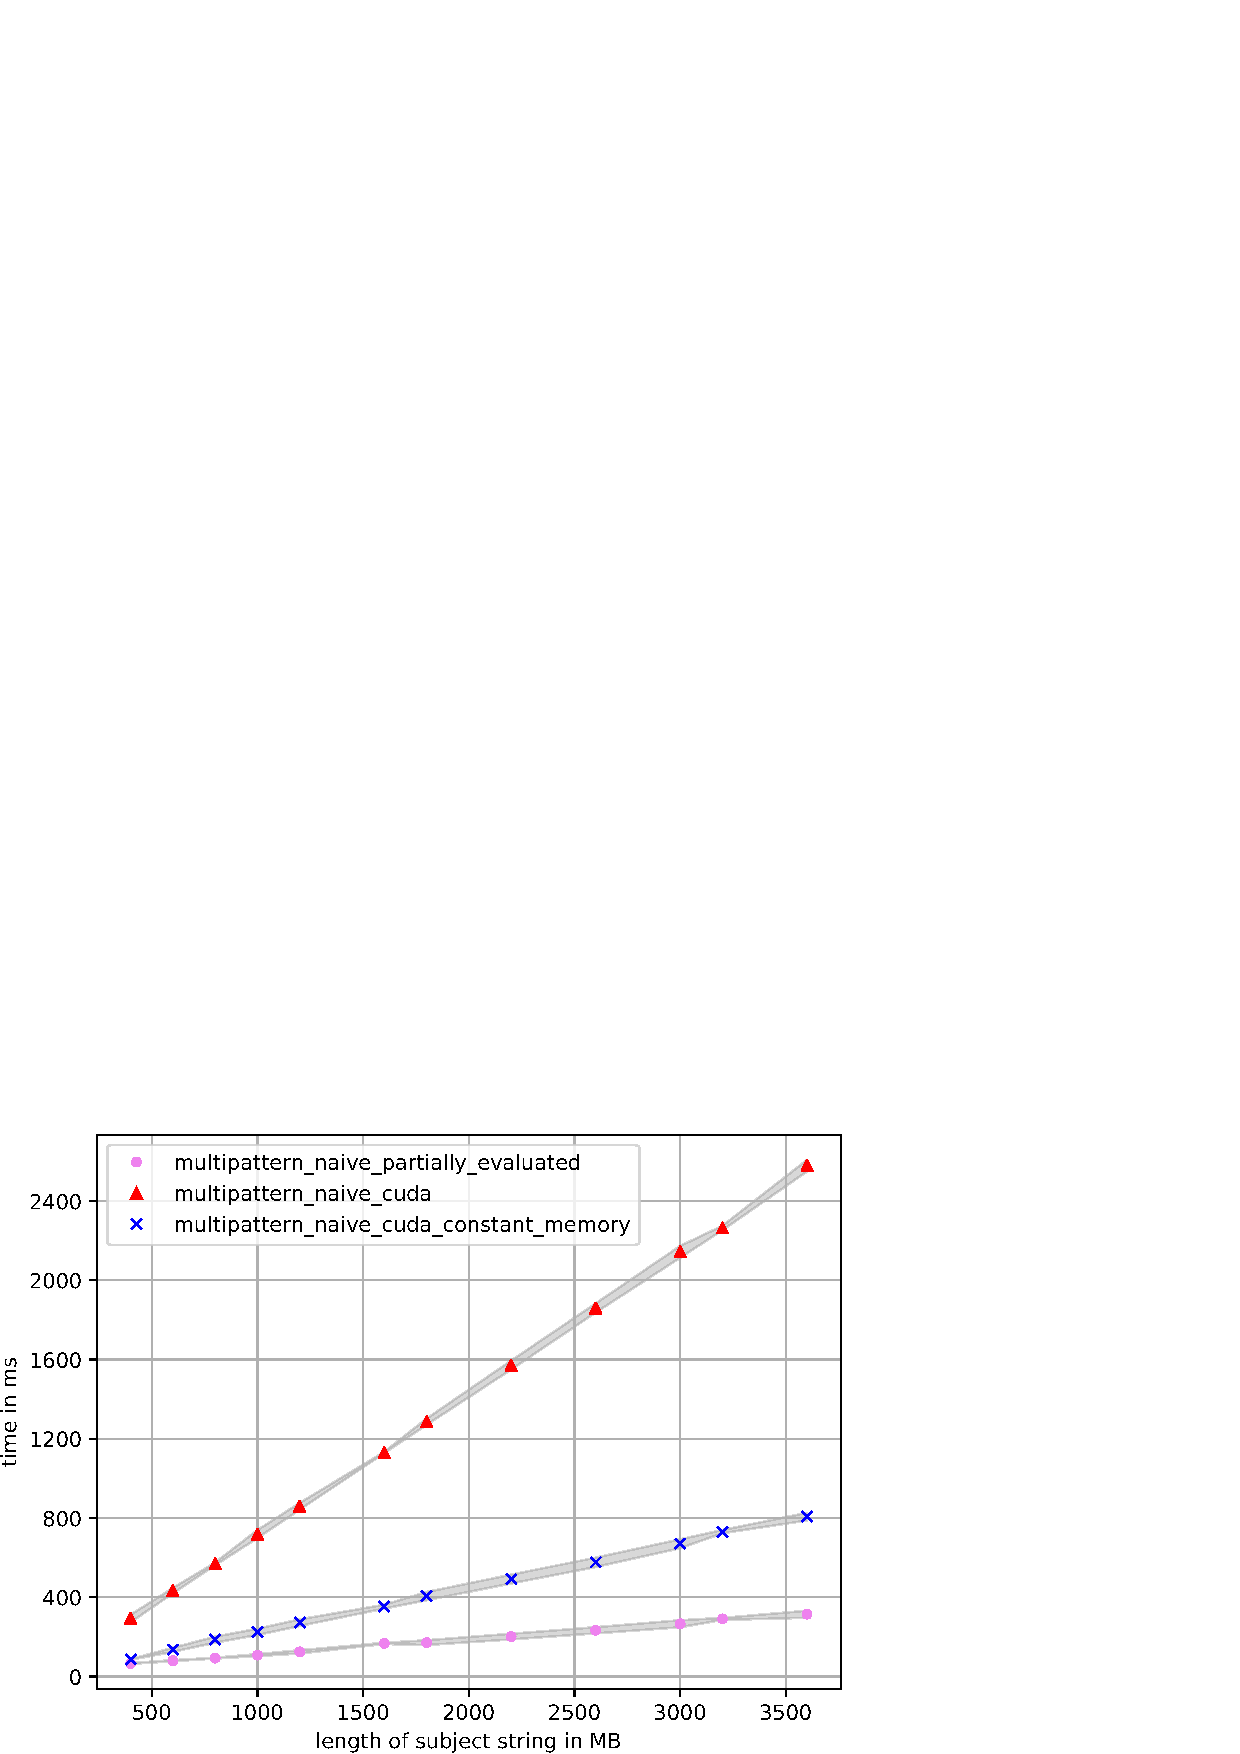
\includegraphics[width=0.9\textwidth]{pictures/results.pdf}}
\end{frame}


\begin{frame}[fragile] \frametitle{Limitations}
  \begin{minipage}[t]{1cm}
\hspace{1cm}
  \end{minipage}
  ~
\begin{minipage}[t]{0.85\textwidth}
\begin{itemize}
\item[\textbf{[RDF]}]
\begin{itemize}
  \item The set of the real-world RDF files (ontologies)
  \item Queries: $G_4: s \to SCOR \ s \ SCO \ | \ TR \ s \ T \ | \ SCOR \ SCO \ | \ TR \ T$
$G_5: s \to SCOR \ s \ SCO \ | \ SCO$
\end{itemize}

\pause
\item[\textbf{[Worst]}]
\begin{itemize}
  \item The input graph is two cycles of coprime lengths with one shared vertex
  \begin{figure}
        \begin{tikzpicture}[shorten >=1pt,node distance=2cm,on grid,auto]
   \node[state] (q_1)   {$1$};
   \node[state] (q_2) [above=of q_1] {$2$};
   \node[state] (q_3) [above right=of q_1, below right=of q_2] {$0$};
   \node[state] (q_4) [right=of q_3] {$3$};
    \path[->]
    (q_1) edge  node {A} (q_2)
    (q_2) edge  node {A} (q_3)
    (q_3) edge  node {A} (q_1)
    (q_3) edge[bend left, above]  node {B} (q_4)
    (q_4) edge[bend left, below]  node {B} (q_3);
\end{tikzpicture}
\end{figure}
  \item Query: $G_1: s \to A \ s \ B \ | \ A \ B$
\end{itemize}
\end{itemize}
\end{minipage}
\end{frame}

\begin{frame}[fragile] \frametitle{Dataset}
  \begin{minipage}[t]{1cm}
\hspace{1cm}
  \end{minipage}
  ~
\begin{minipage}[t]{0.85\textwidth}
\begin{itemize}
\item[\textbf{[Full]}]
\begin{itemize}
  \item The input graph is sparse, but the result is a full graph
  \item Queries: \\ $G_2: s \to s \ s \ | \ A$ \\ $G_3: s \to s \ s \ s \ | \ A$
\end{itemize}
\pause
\item[\textbf{[Sparse]}]
\begin{itemize}
  \item Sparse graphs are generated by GTgraph
  \item Query: $G_1: s \to A \ s \ B \ | \ A \ B$
\end{itemize}
\end{itemize}
\end{minipage}
\end{frame}

\begin{frame} \frametitle{Conclusion}
  \begin{itemize}
   \item Just In Time speciaization
   \item
   \item
   \item
  \end{itemize}
\end{frame}

\begin{frame}[fragile] \frametitle{Future Research}
  \begin{itemize}
    \item Switch to CUDA C partial evaluator
    \begin{itemize}
      \item LLVM.mix: partial evaluator for LLVM IR
    \end{itemize}
    \pause
    \item Reduce specialization overhead
    \begin{itemize}
      \item To be applicable in run-time
    \end{itemize}
    \pause
    \item Integrete with shared memory register spilling
    \begin{itemize}
      \item ``RegDem: Increasing GPU Performance via Shared Memory Register Spilling'' (Putt Sakdhnagool et.al. 2019)
    \end{itemize}
    \pause
    \item Evaluate on real-world examples
  \end{itemize}
\end{frame}

\begin{frame}
\frametitle{Contact Information}
\begin{itemize}
  \item Semyon Grigorev:
    \begin{itemize}
      \item \href{mailto:s.v.grigoriev@spbu.ru}{s.v.grigoriev@spbu.ru}
      \item \href{mailto:Semen.Grigorev@jetbrains.com}{Semen.Grigorev@jetbrains.com}
    \end{itemize}

  \item Aleksey Tyurin: \href{mailto:alekseytyurinspb@gmail.com}{alekseytyurinspb@gmail.com}
  \item Daniil Berezun: \href{mailto:daniil.berezun@jetbrains.com}{daniil.berezun@jetbrains.com}

\vspace{0.5cm}
  \item Dataset and algorithm implementations: \href{https://github.com/SokolovYaroslav/CFPQ-on-GPGPU}{https://github.com/SokolovYaroslav/CFPQ-on-GPGPU}
\end{itemize}
\vspace{0.1cm}
\center{\huge{Thanks!}}
\end{frame}
\end{document}
